\documentclass[12pt]{article}
\usepackage{graphicx}
\usepackage{multirow}
\usepackage{minted}
\usepackage{hyperref}
\setminted{fontsize=\footnotesize}
\usepackage{hyperref}

\title{High-performance Computing, Autumn 2024}
\author{Robert Buj}
\date{\today}

\begin{document}
\maketitle

\section*{Question 1}

\subsection*{1.1}

\begin{figure}[h!]
	\centering
	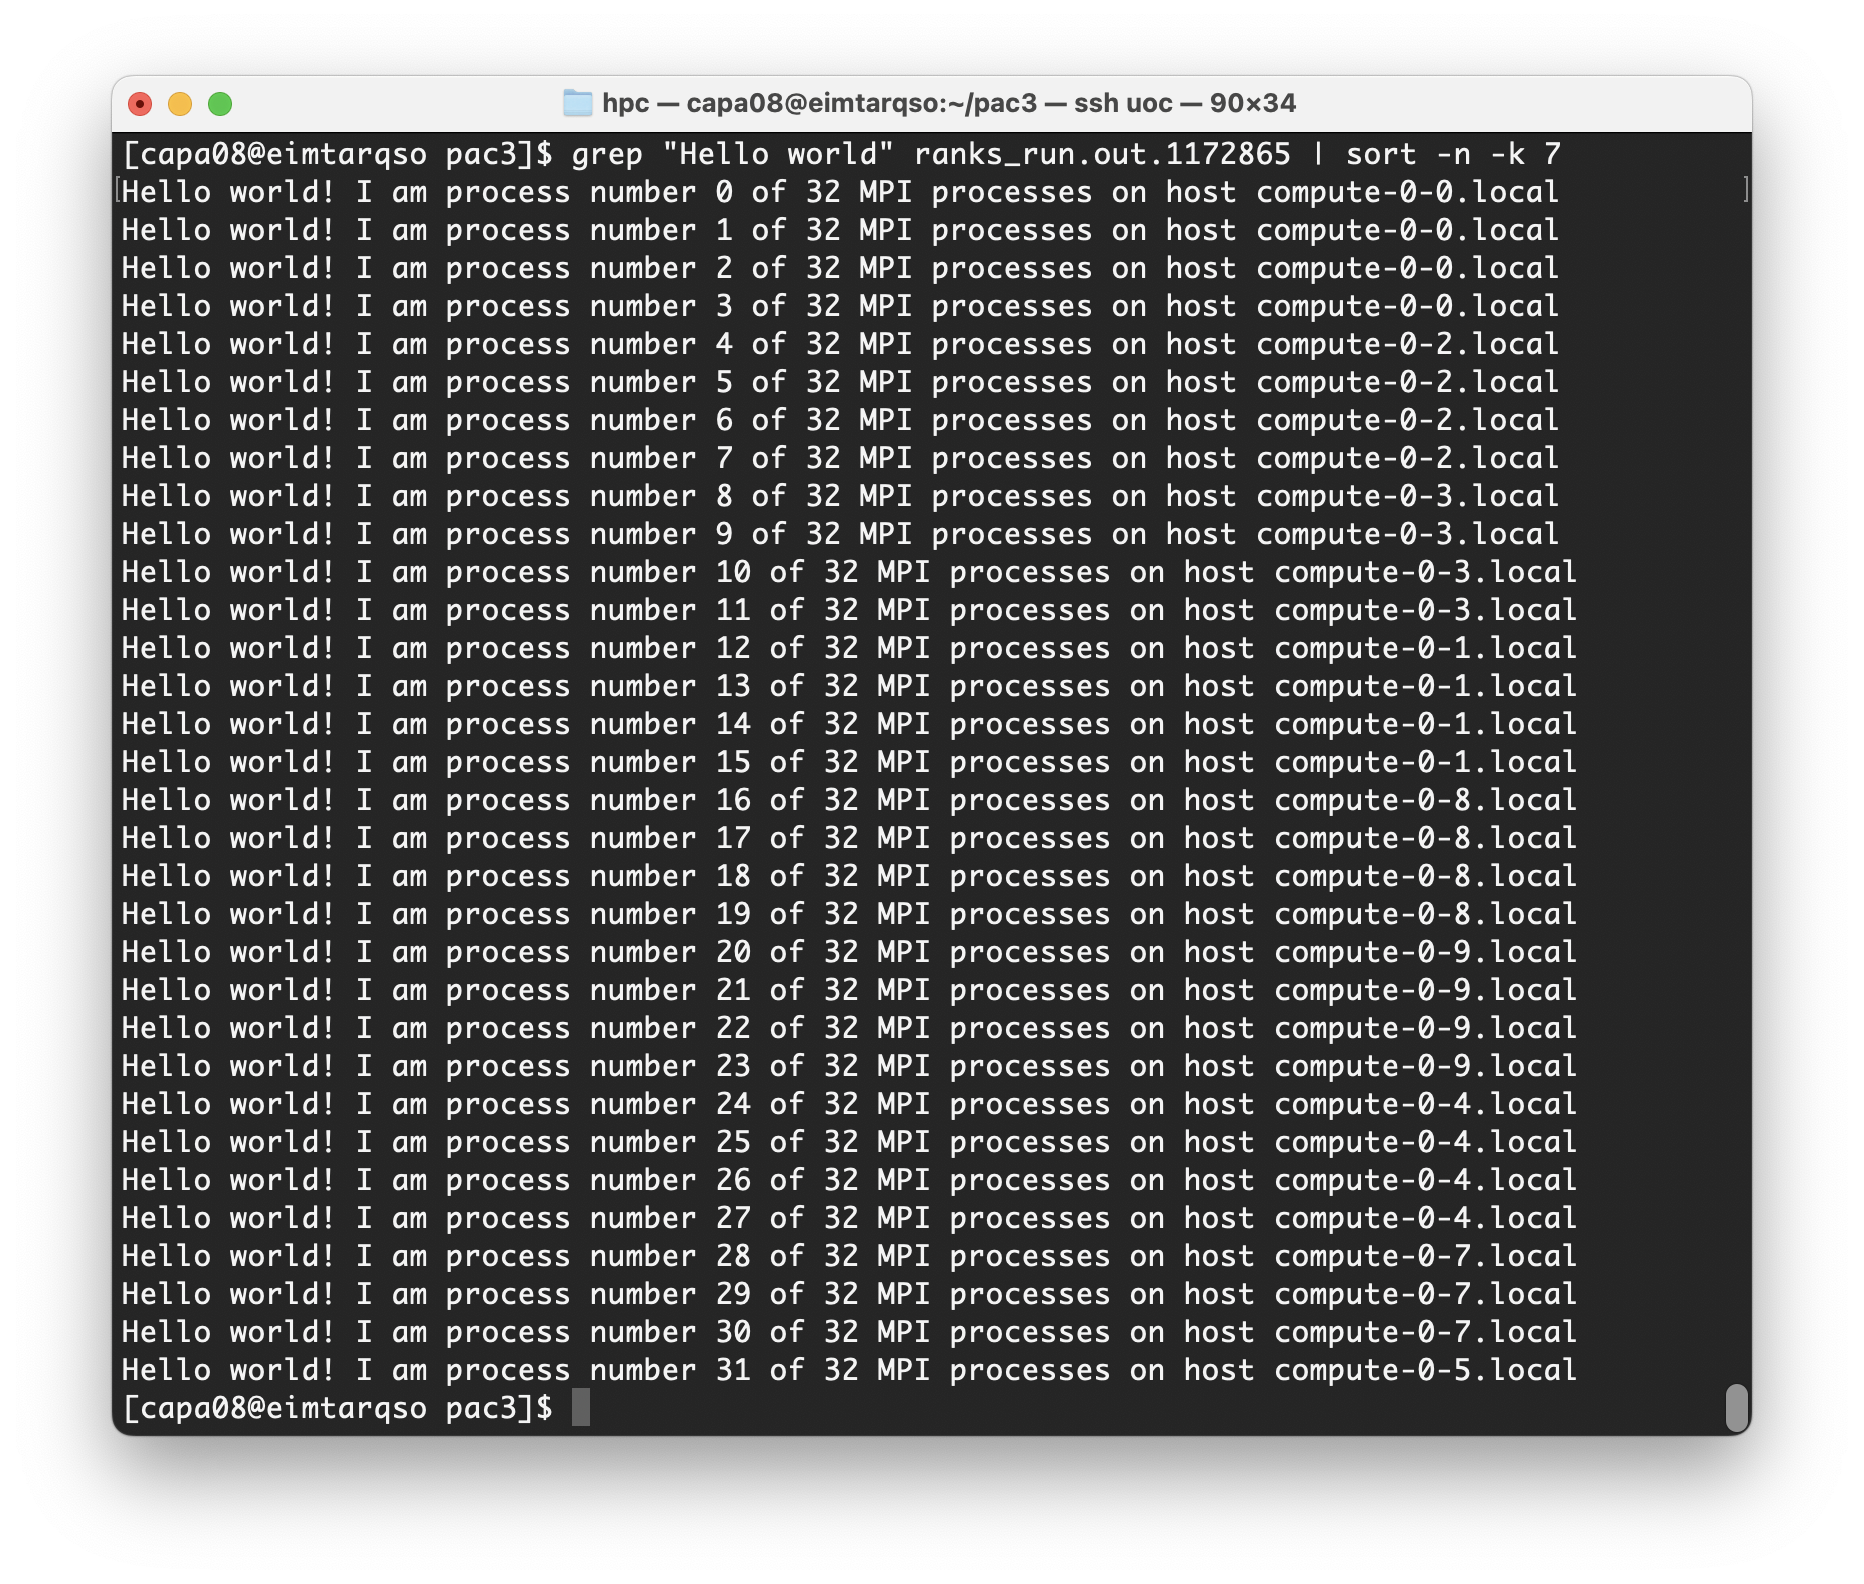
\includegraphics[width=0.8\linewidth]{images/Q1.1.png}
	\caption{Sorted by rank}
	\label{fig:Q1A}
\end{figure}

\newpage

\begin{figure}[h!]
	\begin{minted}{shell}
$ qconf -sp orte
pe_name            orte
slots              9999
user_lists         NONE
xuser_lists        NONE
start_proc_args    /bin/true
stop_proc_args     /bin/true
allocation_rule    $fill_up
control_slaves     TRUE
job_is_first_task  FALSE
urgency_slots      min
accounting_summary TRUE
	\end{minted}
\caption{Get the allocation rule}\label{code:qconf}
\end{figure}

The allocation rule is interpreted by the scheduler thread and helps the scheduler to decide how to distribute parallel processes among the available machines.

\begin{itemize}
	\item \$fill\_up: Starting from the best  suitable  host/queue,  all available  slots  are allocated. Further hosts and queues are "filled up" as  long  as  a  job  still requires slots for parallel tasks.
\end{itemize}

\subsection*{1.2}

I failed to assign statically the ranks to the nodes as they are automatically assigned by SGE.

On the other hand, when using an SGE parallel environment with OpenMPI you no longer have to specify the -np, -hostfile, -host, etc. options to mpirun. This is because SGE will automatically assign hosts and processors to be used by OpenMPI for your job. You also do not need to pass the –byslot and –bynode options to mpirun given that these mechanisms are now handled by the fill\_up and round\_robin modes specified in the SGE parallel environment. REF: \href{http://star.mit.edu/cluster/docs/0.93.3/guides/sge.html}{Sun Grid Engine (SGE) QuickStart, Submitting OpenMPI Jobs using a Parallel Environment}

\newpage

\begin{figure}[h!]
	\centering
	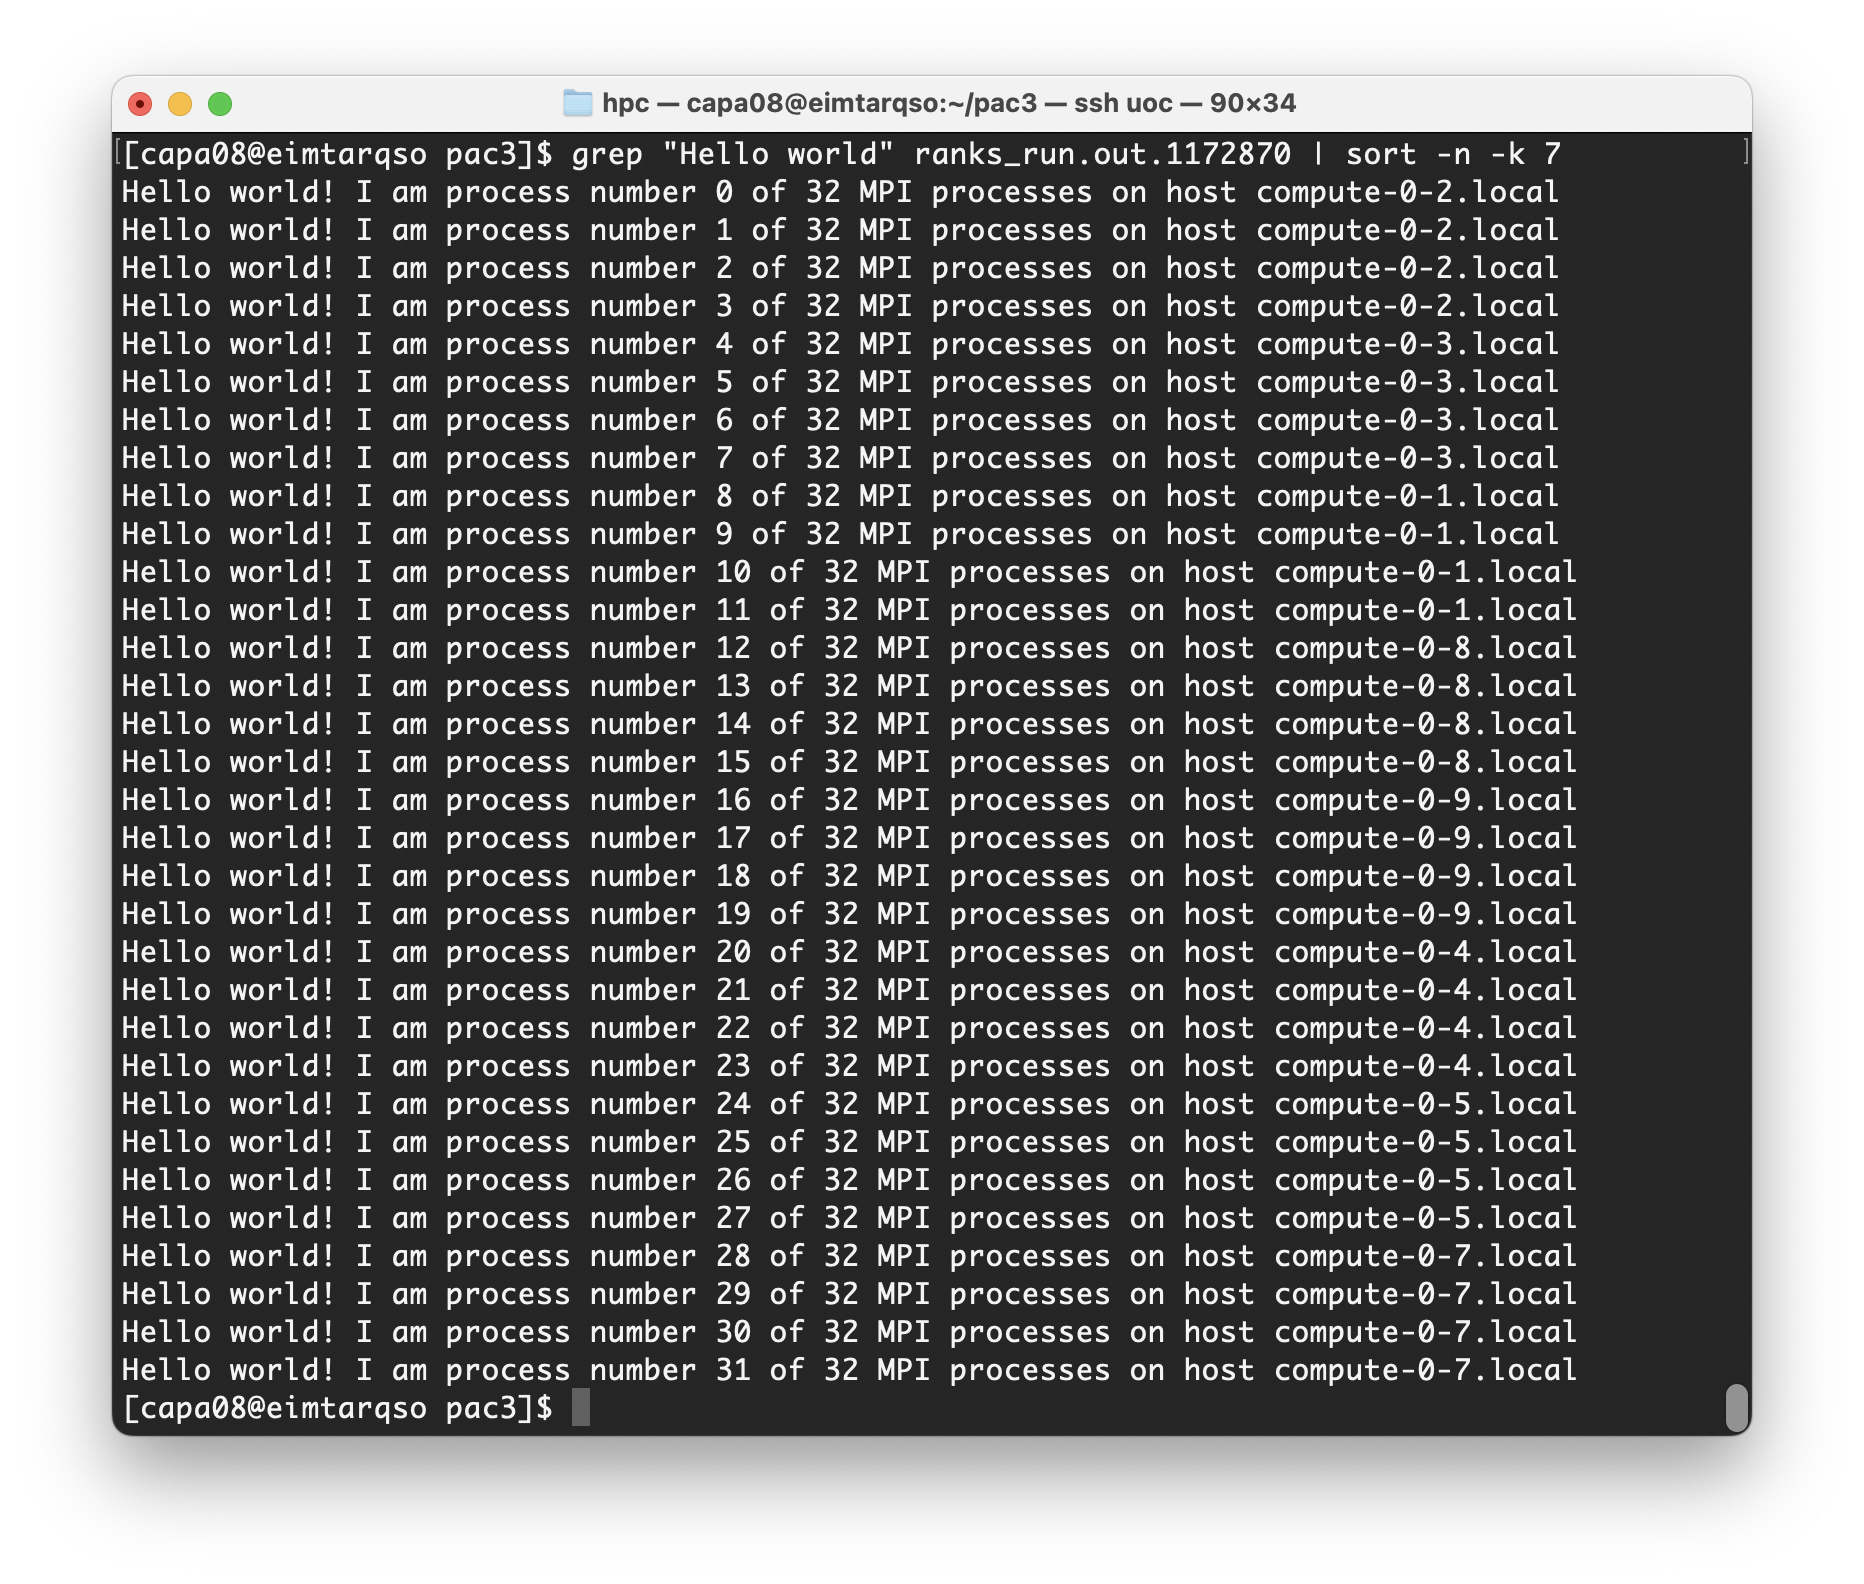
\includegraphics[width=0.8\linewidth]{images/Q1.2.png}
	\caption{Sorted by rank, 2nd run}
	\label{fig:Q1B}
\end{figure}

\section*{Question 2}

\subsection*{2.1}

There is a deadlock because the application makes use of the schema, send and then receive the message to each other, and both are sending large messages, which are sent in synchronous mode. It means that both ranks are blocked waiting for the acknowledgement after sending the message, and for this reason they can't run the next sentence to receive the message from partner.

\begin{figure}[h!]
	\begin{minted}{shell}
Rank 0 is reported
Rank size: 2
Rank 1 is reported
	\end{minted}
\caption{Output of deadlock execution}\label{code:build}
\end{figure}

\subsection*{2.2}

There is no deadlock, as small messages are catched and stored by the recepient into an auxiliar buffer who send the acknowledgement to the sender, so the applicion continues its execution on both ranks.

\begin{figure}[h!]
	\begin{minted}{shell}
Rank 0 is reported
Rank size: 2
Rank 0 sends to 1
Rank 0 receives from 1
Rank 1 is reported
Rank 1 sends to 0
Rank 1 receives from 0
	\end{minted}
	\caption{Output of deadlock execution with smaller size, SIZE=1024}\label{code:build}
\end{figure}

I couldn't figure out how to reproduce the same behaviour with short messages. I tried to fulfill the buffer to force synchronous messages without success. See deadlock.SIZE.v2.c

\begin{figure}[h!]
	\begin{minted}{C}
...
#define N 100000
...
  if (rank == 0) {
    int partner = 1;
    for (unsigned int i=0;i<N;i++) {
      MPI_Send(v1, SIZE, MPI_INT, partner, 100, MPI_COMM_WORLD);
      printf("Rank %d sends to %d\n", rank, partner);
    }
...
  } else if (rank == 1) {
    int partner = 0;
    for (unsigned int i=0;i<N;i++) {
      MPI_Send(v1, SIZE, MPI_INT, partner, 100, MPI_COMM_WORLD);
      printf("Rank %d sends to %d\n", rank, partner);
    }
...
	\end{minted}
	\caption{source/src/deadlock.SIZE.v2.c}\label{code:size2}
\end{figure}

\newpage

\subsection*{2.3}

Option 2: For one of the ranks, swap MPI\_Send and MPI\_Recv, for instance rank 1.

\begin{figure}[h!]
	\begin{minted}{C}
if (rank == 0) {
  int partner = 1;
  MPI_Send(v1, SIZE, MPI_INT, partner, 100, MPI_COMM_WORLD);
  printf("Rank %d sends to %d\n", rank, partner);
  MPI_Recv(v2, SIZE, MPI_INT, partner, 100, MPI_COMM_WORLD, MPI_STATUS_IGNORE);
  printf("Rank %d receives from %d\n", rank, partner);
} else if (rank == 1) {
  int partner = 0;
  MPI_Recv(v2, SIZE, MPI_INT, partner, 100, MPI_COMM_WORLD, MPI_STATUS_IGNORE);
  printf("Rank %d receives from %d\n", rank, partner);
  MPI_Send(v1, SIZE, MPI_INT, partner, 100, MPI_COMM_WORLD);
  printf("Rank %d sends to %d\n", rank, partner);
}
	\end{minted}
	\caption{source/src/deadlock.2.c}\label{code:build}
\end{figure}

The user numeric part modulo 3 is 2.

\begin{figure}[h!]
	\begin{minted}{shell}
		$ whoami 
		capa08
		$ echo 8 % 3 | bc
		2
	\end{minted}
	\caption{get the username and option number from its numerical part}\label{code:user}
\end{figure}

The other two options have also been implemented:

\begin{itemize}
	\item Option 0: Non-blocking communications: source/src/deadlock.0.c
	\item Option 1:	“Chain” sending operations (MPI Sendrecv): source/src/deadlock.1.c
\end{itemize}

\newpage

\subsection*{2.4}

As it's shown in the figure below, both ranks ran the same sentences in the same order, except MPI\_Send and MPI\_Recv which are swapped on rank 1 (THREAD 1.2.1).

Rank 1 started listening before rank 0 (THREAD 1.2.1) started sending the message. It doesn't matter much, because in case of node 1 wasn't ready, the message would be sent again after a timeout.

Rank 0 sent the entire message to rank 1. Rank 1 received the message and it sent the acknowledgement to rank 0, and it started to read the message.

Rank 1, after receiving the acknowledgement from node 0, started listening. Rank 0, after reading the message sent by node 0, started to send to rank 1 its own message.

Rank 0, after receiving the message from rank 0, sent an acknowledgement to rank 1. Rank 1 received the acknowledgement and started the MPI\_Finalize. Rank 0 completed the reading of the message and started the MPI\_Finalize.

\begin{figure}[h!]
	\centering
	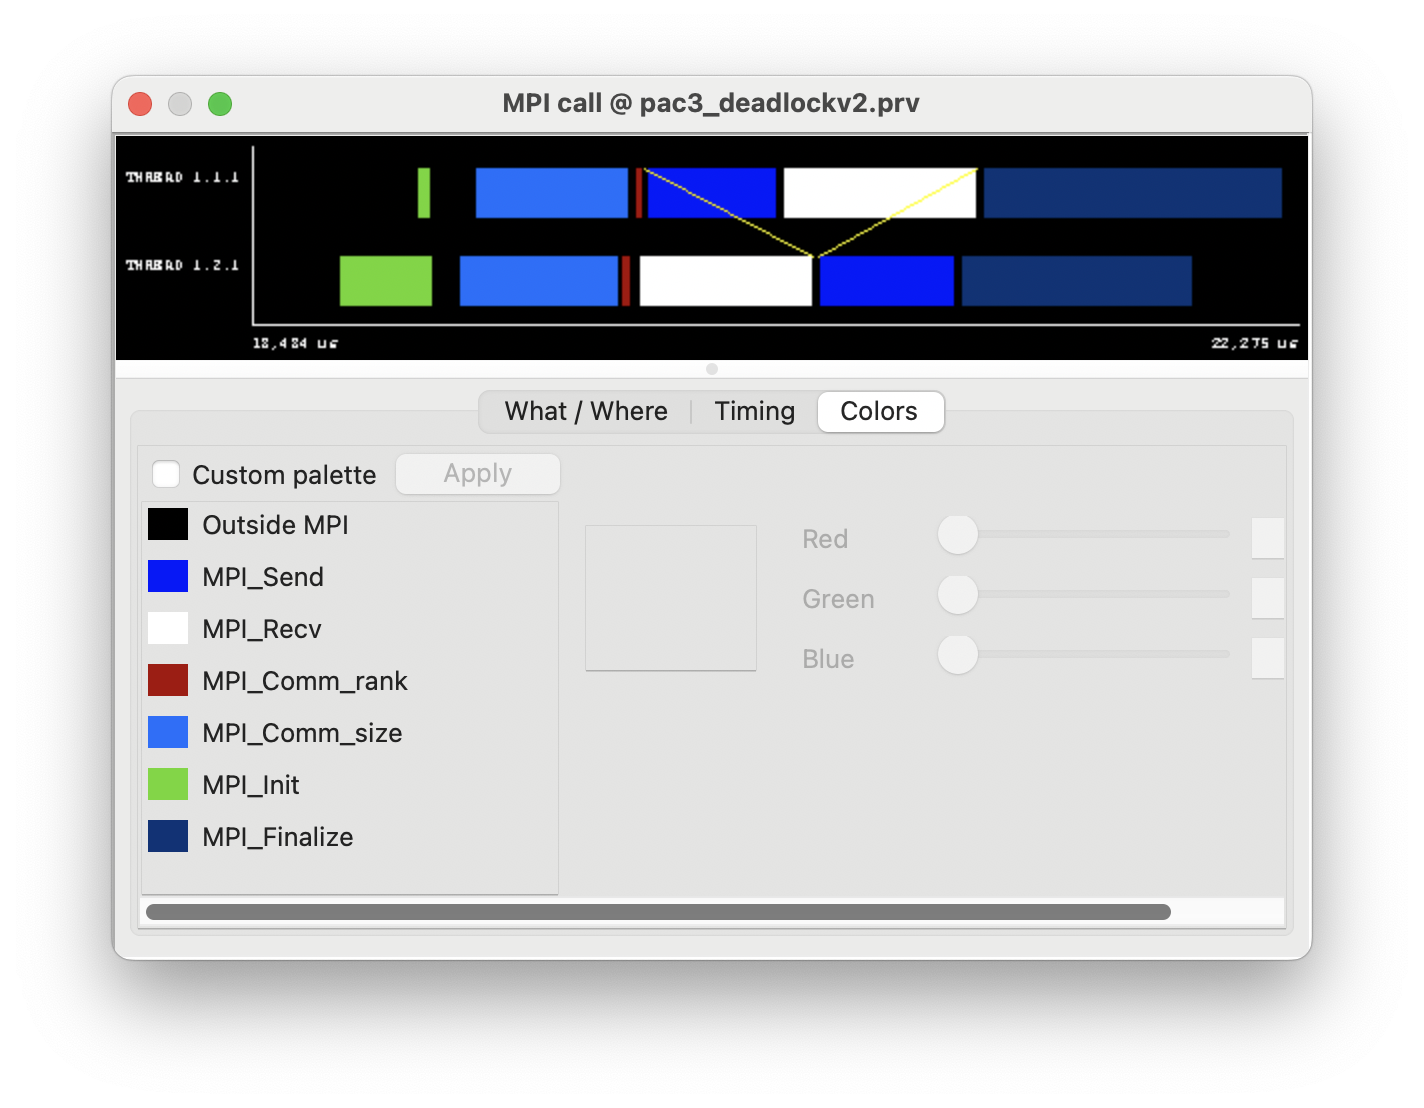
\includegraphics[width=0.8\linewidth]{images/paraver.o2.colors.png}
	\caption{Trace of option 2: swap send and receive on rank 1}
	\label{fig:swap}
\end{figure}

\newpage

\section*{Question 3}

\begin{figure}[h!]
	\centering
	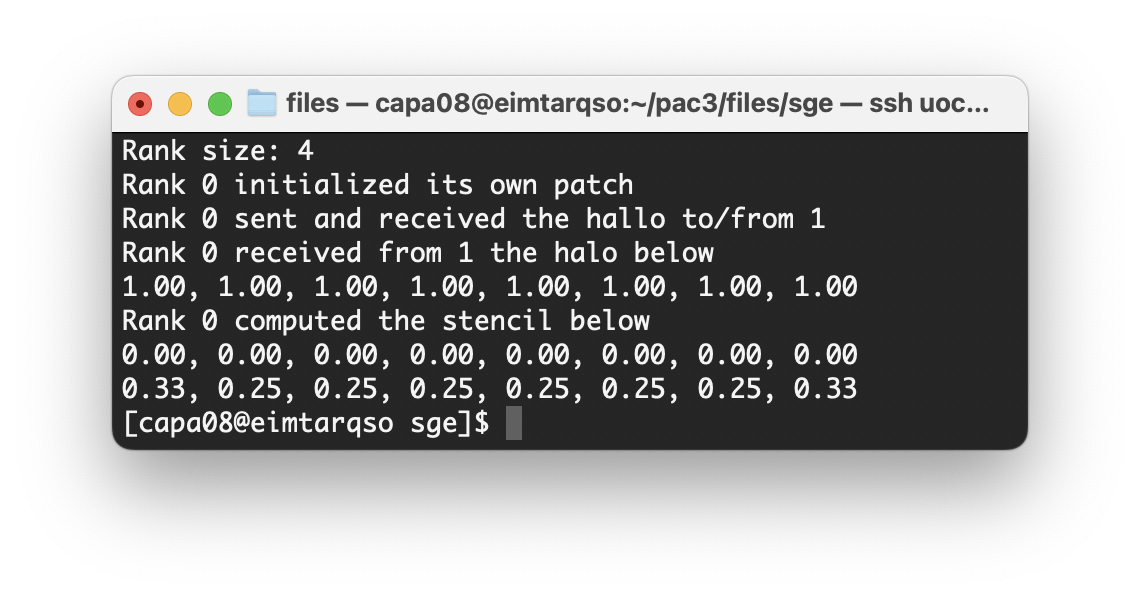
\includegraphics[width=0.8\linewidth]{images/Q3.png}
	\caption{Screenshot of the execution}
	\label{fig:stencil}
\end{figure}

The user numeric part modulo 4 is 0.

\begin{figure}[h!]
	\begin{minted}{shell}
		$ whoami 
		capa08
		$ echo 8 % 4 | bc
		0
	\end{minted}
	\caption{get the username and option number from its numerical part}\label{code:user}
\end{figure}

Two approaches have been used for halo exchange.
The patches at the top and at the bottom use MPI\_Sendrecv, because they only have one adjacent patch and they only have to send and receive on halo each one.
\begin{figure}[h!]
	\begin{minted}{C}
/* exchange the halos */
MPI_Sendrecv(x[ROWS - 1], COLS, MPI_DOUBLE, partner, 100,
	halo, COLS, MPI_DOUBLE, partner, 100,
	MPI_COMM_WORLD, MPI_STATUS_IGNORE);
	\end{minted}
	\caption{patch at the top}\label{code:extrem}
\end{figure}

\newpage

On the other hand, the other patches have two adjacent patches, and they have to send and receive two halos to/from their adjacent patches. In this case, the halos are exchanged by using non blocking sentences and they wait for the completion. 

\begin{figure}[h!]
	\begin{minted}{C}
/* exchange the halos */
MPI_Isend(x[1], COLS, MPI_DOUBLE, partners[0], 100,
	MPI_COMM_WORLD, &requests[0]);
MPI_Isend(x[2], COLS, MPI_DOUBLE, partners[1], 100,
	MPI_COMM_WORLD, &requests[1]);
MPI_Irecv(halos[0], COLS, MPI_DOUBLE, partners[0], 100,
	MPI_COMM_WORLD, &requests[2]);
MPI_Irecv(halos[1], COLS, MPI_DOUBLE, partners[1], 100,
	MPI_COMM_WORLD, &requests[3]);
MPI_Waitall(4, requests, MPI_STATUSES_IGNORE);
	\end{minted}
\caption{inter patches}\label{code:inter}
\end{figure}

\section*{Question 4}

\begin{figure}[h!]
	\centering
	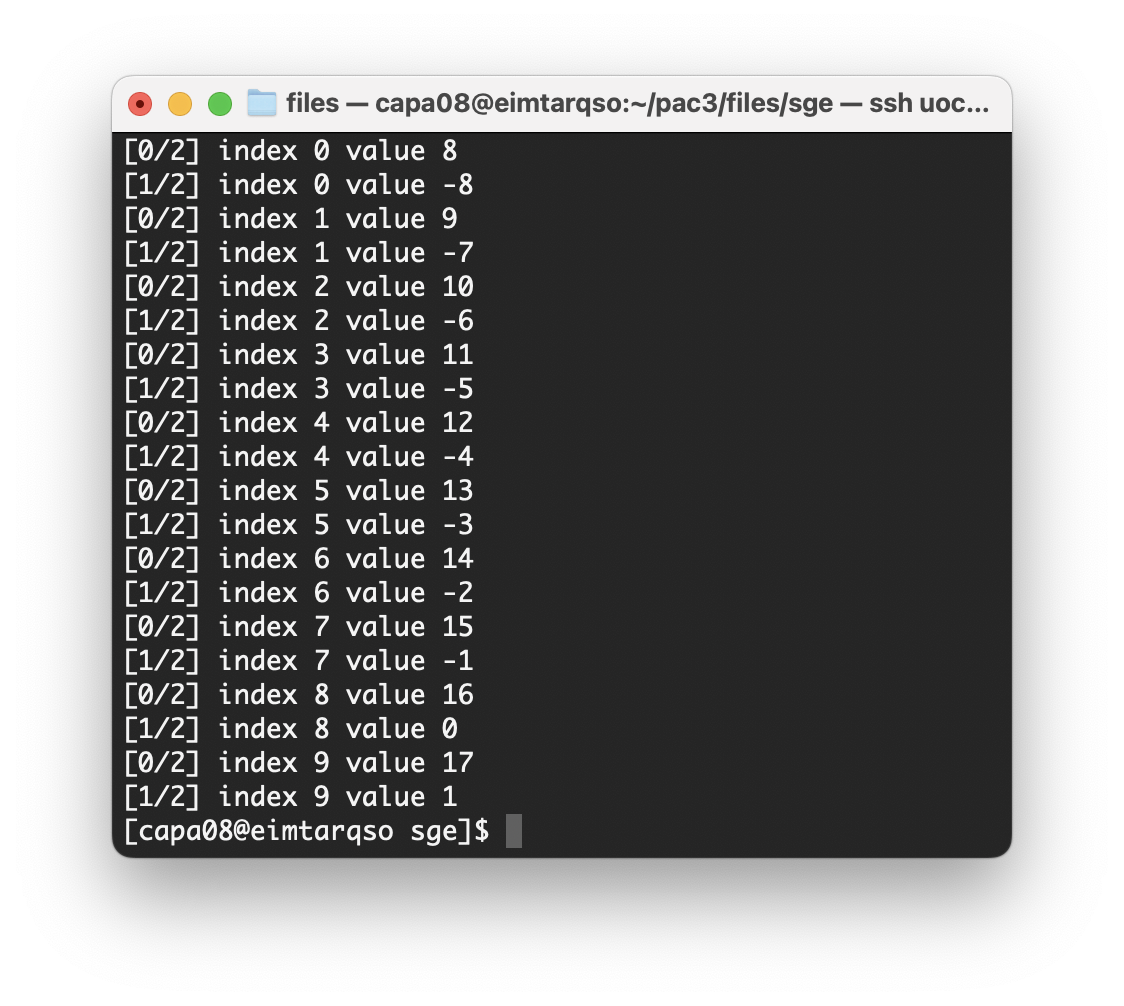
\includegraphics[width=0.6\linewidth]{images/Q4.png}
	\caption{Screenshot of the execution}
	\label{fig:scr04}
\end{figure}

The numerical part of the userid is 8.

\begin{figure}[h!]
	\begin{minted}{shell}
$ whoami 
capa08
	\end{minted}
	\caption{get the numerical part from the userid}\label{code:user}
\end{figure}

\newpage

\section*{List of commands}

\begin{figure}[h!]
	\begin{minted}{shell}
cd source
./autogen.sh 
./configure --prefix=$HOME
make
make install
	\end{minted}
	\caption{Get binaries from source and install them on \$HOME/bin folder which is on \$PATH environment variable}\label{code:build}
\end{figure}

\begin{figure}[h!]
	\begin{minted}{shell}
# .bash_profile

# Get the aliases and functions
if [ -f ~/.bashrc ]; then
. ~/.bashrc
fi

# User specific environment and startup programs

PATH=$PATH:/share/apps/gnuplot/bin:$HOME/bin

export PATH

echo "$(uname -n) says"
cat << EOF
_          _ _       
| |        | | |      
| |__   ___| | | ___  
| '_ \ / _ \ | |/ _ \ 
| | | |  __/ | | (_) |
|_| |_|\___|_|_|\___/ 

EOF
	\end{minted}
	\caption{Content of ~/.bash\_profile}\label{code:bashrc}
\end{figure}

\newpage

\begin{figure}[h!]
	\begin{minted}{shell}
cd sge; qsub ranks.sge; qsub ranks.sge
grep "Hello world" ranks_run.out.1172865 | sort -n -k 7
grep "Hello world" ranks_run.out.1172870 | sort -n -k 7
	\end{minted}
\caption{Question 1}\label{code:q1}
\end{figure}

\begin{figure}[h!]
	\begin{minted}{shell}
cd sge
BASEDIR=$PWD
qsub mpi_send_recv.sge
cd trace/mpi_send_recv
cp /share/apps/extrae/share/example/MPI/extrae.xml ./
cp ~/bin/pac3_mpi_send_recv ./
qsub mpi_send_recv.extrae.sge
cd $BASEDIR
qsub deadlock.sge
qsub qsub deadlockv0.sge
qsub qsub deadlockv1.sge
qsub qsub deadlockv2.sge
cd $BASEDIR
cd trace/deadlockv0
cp /share/apps/extrae/share/example/MPI/extrae.xml ./
qsub deadlockv0.extrae.sge
cd $BASEDIR
cd trace/deadlockv1
cp /share/apps/extrae/share/example/MPI/extrae.xml ./
qsub deadlockv1.extrae.sge
cd $BASEDIR
cd trace/deadlockv2
cp /share/apps/extrae/share/example/MPI/extrae.xml ./
qsub deadlockv2.extrae.sge
	\end{minted}
\caption{Question 2}\label{code:q2}
\end{figure}

\begin{figure}[h!]
	\begin{minted}{shell}
cd sge
qsub stencil.sge
	\end{minted}
	\caption{Question 3}\label{code:q3}
\end{figure}

\newpage

\begin{figure}[h!]
	\begin{minted}{shell}
cd sge
qsub rma.sge
	\end{minted}
	\caption{Question 4}\label{code:q4}
\end{figure}

\newpage

\section*{File Content}
\subsection*{Source Files}

\begin{figure}[h!]
	\begin{minted}{C}
#include "mpi.h"
#include <stdio.h>
#include <stdlib.h> /* EXIT_SUCCESS */
#include <unistd.h>

int main(int argc, char **argv)
{
  int rank, numprocs;
  char hostname[256];
	
  MPI_Init(&argc,&argv);
  MPI_Comm_rank(MPI_COMM_WORLD, &rank);
  MPI_Comm_size(MPI_COMM_WORLD, &numprocs);
  gethostname(hostname,255);
  printf("Hello world! I am process number %d of %d MPI processes on host %s\n",
  rank, numprocs, hostname);
  MPI_Finalize();
  return EXIT_SUCCESS;
}
	\end{minted}
\caption{source/src/ranks.c }\label{code:ranksc}
\end{figure}

\newpage

\begin{figure}[h!]
	\begin{minted}{C}
#include "mpi.h"
#include <stdio.h>
#include <stdlib.h> /* EXIT_SUCCESS */

int main(int argc, char* argv[]) {
  int MyProc, tag=1;
  char msg='A', msg_recpt;
  MPI_Status status;
	
  MPI_Init(&argc, &argv);
  MPI_Comm_rank(MPI_COMM_WORLD, &MyProc);

  printf("Process # %d started \n", MyProc);
  MPI_Barrier(MPI_COMM_WORLD);

  if (MyProc == 0) {
    printf("Sending message to Proc #1 \n") ;
    MPI_Send(&msg, 1, MPI_CHAR, 1, tag, MPI_COMM_WORLD);
    MPI_Recv(&msg_recpt, 1, MPI_CHAR, 1, tag, MPI_COMM_WORLD, &status);
    printf("Recv'd message from Proc #1 \n") ;
  } else {
    MPI_Recv(&msg_recpt, 1, MPI_CHAR, 0, tag, MPI_COMM_WORLD, &status);
    printf("Recv'd message from Proc #0 \n") ;
    printf("Sending message to Proc #0 \n") ;
    MPI_Send(&msg, 1, MPI_CHAR, 0, tag, MPI_COMM_WORLD);
  }
  printf("Finishing proc %d\n", MyProc); 
  MPI_Barrier(MPI_COMM_WORLD); 
  MPI_Finalize();
  return EXIT_SUCCESS;
}
	\end{minted}
	\caption{source/src/mpi\_send\_recv.c}\label{code:sandrc}
\end{figure}

\newpage

\begin{figure}[h!]
	\begin{minted}{C}
#include "mpi.h" /* MPI_Init, MPI_Finalize, MPI_Send, MPI_Recv,
MPI_Comm_size, MPI_Comm_rank, MPI_COMM_WORLD, MPI_STATUS_IGNORE */
#include <stdio.h>
#include <stdlib.h> /* EXIT_SUCCESS */
#define SIZE 100000

int main(int argc, char* argv[]){
  MPI_Init(&argc, &argv);

  int size;
  MPI_Comm_size(MPI_COMM_WORLD, &size);

  /* Get my rank */
  int rank;
  MPI_Comm_rank(MPI_COMM_WORLD, &rank);
  printf("Rank %d is reported\n", rank);
  if (rank == 0) printf("Rank size: %d\n", size);
  int v1[SIZE];
  int v2[SIZE];
  if (rank == 0) {
    int partner = 1;
    MPI_Send(v1, SIZE, MPI_INT, partner, 100, MPI_COMM_WORLD);
    printf("Rank %d sends to %d\n", rank, partner);
    MPI_Recv(v2, SIZE, MPI_INT, partner, 100, MPI_COMM_WORLD,
             MPI_STATUS_IGNORE);
    printf("Rank %d receives from %d\n", rank, partner);
  } else if (rank == 1) {
    int partner = 0;
    MPI_Send(v1, SIZE, MPI_INT, partner, 100, MPI_COMM_WORLD);
    printf("Rank %d sends to %d\n", rank, partner);
    MPI_Recv(v2, SIZE, MPI_INT, partner, 100, MPI_COMM_WORLD,
             MPI_STATUS_IGNORE);
    printf("Rank %d receives from %d\n", rank, partner);
  }
  MPI_Finalize();
  return EXIT_SUCCESS;
}
	\end{minted}
	\caption{source/src/deadlock.c}\label{code:deadlockc}
\end{figure}

\newpage

\begin{figure}[h!]
	\begin{minted}{C}
#include <mpi.h>
#include <stdio.h>
#include <stdlib.h> /* EXIT_SUCCESS */

int main(int argc, char* argv[]){
  MPI_Init(&argc, &argv);

  int size, rank;
  MPI_Comm_size(MPI_COMM_WORLD, &size);
  MPI_Comm_rank(MPI_COMM_WORLD, &rank);
  printf("Rank %d is reported\n", rank);
  if (rank == 0) printf("Rank size: %d\n", size);
  int v1[SIZE];
  int v2[SIZE];
  if (rank == 0) {
    int partner = 1;
    MPI_Send(v1, SIZE, MPI_INT, partner, 100, MPI_COMM_WORLD);
    printf("Rank %d sends to %d\n", rank, partner);
    MPI_Recv(v2, SIZE, MPI_INT, partner, 100, MPI_COMM_WORLD,
             MPI_STATUS_IGNORE);
    printf("Rank %d receives from %d\n", rank, partner);
  } else if (rank == 1) {
    int partner = 0;
    MPI_Send(v1, SIZE, MPI_INT, partner, 100, MPI_COMM_WORLD);
    printf("Rank %d sends to %d\n", rank, partner);
    MPI_Recv(v2, SIZE, MPI_INT, partner, 100, MPI_COMM_WORLD,
             MPI_STATUS_IGNORE);
    printf("Rank %d receives from %d\n", rank, partner);
  }
  MPI_Finalize();
  return 0;
}
	\end{minted}
	\caption{source/src/deadlock.SIZE.c}\label{code:deadlockSc}
\end{figure}

\newpage

\begin{figure}[h!]
	\begin{minted}{C}
#include <mpi.h>
#include <stdio.h>
#include <stdlib.h> /* EXIT_SUCCESS */
#define N 100000

int main(int argc, char* argv[]){
  MPI_Init(&argc, &argv);

  int size, rank;
  MPI_Comm_size(MPI_COMM_WORLD, &size);
  MPI_Comm_rank(MPI_COMM_WORLD, &rank);
  printf("Rank %d is reported\n", rank);
  if (rank == 0) printf("Rank size: %d\n", size);
  int v1[SIZE];
  int v2[SIZE];
  if (rank == 0) {
    int partner = 1;
    for (unsigned int i=0;i<N;i++) {
      MPI_Send(v1, SIZE, MPI_INT, partner, 100, MPI_COMM_WORLD);
      printf("Rank %d sends to %d\n", rank, partner);
    }
    for (unsigned int i=0;i<N;i++) {
      MPI_Recv(v2, SIZE, MPI_INT, partner, 100, MPI_COMM_WORLD,
               MPI_STATUS_IGNORE);
      printf("Rank %d receives from %d\n", rank, partner);
    }
  } else if (rank == 1) {
    int partner = 0;
    for (unsigned int i=0;i<N;i++) {
      MPI_Send(v1, SIZE, MPI_INT, partner, 100, MPI_COMM_WORLD);
      printf("Rank %d sends to %d\n", rank, partner);
    }
    for (unsigned int i=0;i<N;i++) {
      MPI_Recv(v2, SIZE, MPI_INT, partner, 100, MPI_COMM_WORLD,
               MPI_STATUS_IGNORE);
      printf("Rank %d receives from %d\n", rank, partner);
    }
  }
  MPI_Finalize();
  return 0;
}
	\end{minted}
	\caption{source/src/deadlock.SIZE.v2.c}\label{code:deadlockSc}
\end{figure}

\newpage

\begin{figure}[h!]
	\begin{minted}{C}
#include "mpi.h" /* MPI_Init, MPI_Finalize, MPI_Isend, MPI_Irecv,
                    MPI_Waitall, MPI_Comm_size, MPI_Comm_rank,
                    MPI_Request, MPI_COMM_WORLD, MPI_STATUSES_IGNORE */
#include <stdio.h>
#include <stdlib.h> /* EXIT_SUCCESS */
#define SIZE 100000

int main(int argc, char* argv[]){
  MPI_Init(&argc, &argv);

  int size;
  MPI_Comm_size(MPI_COMM_WORLD, &size);

  /* Get my rank */
  int rank;
  MPI_Comm_rank(MPI_COMM_WORLD, &rank);
  printf("Rank %d is reported\n", rank);
  if (rank == 0) printf("Rank size: %d\n", size);

  int v1[SIZE];
  int v2[SIZE];
  MPI_Request requests[2];
  if (rank == 0) {
    int partner = 1;
    MPI_Isend(v1, SIZE, MPI_INT, partner, 100, MPI_COMM_WORLD, &requests[0]);
    MPI_Irecv(v2, SIZE, MPI_INT, partner, 100, MPI_COMM_WORLD, &requests[1]);
    MPI_Waitall(2, requests, MPI_STATUSES_IGNORE);
    printf("Rank %d sends to %d\n", rank, partner);
    printf("Rank %d receives from %d\n", rank, partner);
  } else if (rank == 1) {
    int partner = 0;
    MPI_Isend(v1, SIZE, MPI_INT, partner, 100, MPI_COMM_WORLD, &requests[0]);
    MPI_Irecv(v2, SIZE, MPI_INT, partner, 100, MPI_COMM_WORLD, &requests[1]);
    MPI_Waitall(2, requests, MPI_STATUSES_IGNORE);
    printf("Rank %d sends to %d\n", rank, partner);
    printf("Rank %d receives from %d\n", rank, partner);
  }
  MPI_Finalize();
  return EXIT_SUCCESS;
}
	\end{minted}
	\caption{source/src/deadlock.0.c}\label{code:deadlockc}
\end{figure}

\newpage

\begin{figure}[h!]
	\begin{minted}{C}
#include "mpi.h" /* MPI_Init, MPI_Finalize, MPI_Sendrecv, MPI_Comm_size,
MPI_Comm_rank, MPI_COMM_WORLD, MPI_STATUS_IGNORE */
#include <stdio.h>
#include <stdlib.h> /* EXIT_SUCCESS */
#define SIZE 100000

int main(int argc, char *argv[]) {
  MPI_Init(&argc, &argv);

  int size;
  MPI_Comm_size(MPI_COMM_WORLD, &size);
	
  /* Get my rank */
  int rank;
  MPI_Comm_rank(MPI_COMM_WORLD, &rank);
  printf("Rank %d is reported\n", rank);
  if (rank == 0) printf("Rank size: %d\n", size);
 
  int v1[SIZE];
  int v2[SIZE];
  if (rank == 0) {
    int partner = 1;
    MPI_Sendrecv(v1, SIZE, MPI_INT, partner, 100,
                 v2, SIZE, MPI_INT, partner, 100,
		         MPI_COMM_WORLD, MPI_STATUS_IGNORE);
    printf("Rank %d sends to %d\n", rank, partner);
    printf("Rank %d receives from %d\n", rank, partner);
  } else if (rank == 1) {
    int partner = 0;
    MPI_Sendrecv(v1, SIZE, MPI_INT, partner, 100,
                 v2, SIZE, MPI_INT, partner, 100,
                 MPI_COMM_WORLD, MPI_STATUS_IGNORE);
    printf("Rank %d sends to %d\n", rank, partner);
    printf("Rank %d receives from %d\n", rank, partner);
  }
  MPI_Finalize();
  return EXIT_SUCCESS;
}
	\end{minted}
	\caption{source/src/deadlock.1.c}\label{code:deadlockc}
\end{figure}

\newpage

\begin{figure}[h!]
	\begin{minted}{C}
#include "mpi.h" /* MPI_Init, MPI_Finalize, MPI_Send, MPI_Recv,
                    MPI_Comm_size, MPI_Comm_rank */
#include <stdio.h>
#include <stdlib.h> /* EXIT_SUCCESS */
#define SIZE 100000

int main(int argc, char* argv[]){
  MPI_Init(&argc, &argv);

  int size;
  MPI_Comm_size(MPI_COMM_WORLD, &size);

  /* Get my rank */
  int rank;
  MPI_Comm_rank(MPI_COMM_WORLD, &rank);
  printf("Rank %d is reported\n", rank);
  if (rank == 0) printf("Rank size: %d\n", size);

  int v1[SIZE];
  int v2[SIZE];
  if (rank == 0) {
    int partner = 1;
    MPI_Send(v1, SIZE, MPI_INT, partner, 100, MPI_COMM_WORLD);
    printf("Rank %d sends to %d\n", rank, partner);
    MPI_Recv(v2, SIZE, MPI_INT, partner, 100, MPI_COMM_WORLD,
             MPI_STATUS_IGNORE);
    printf("Rank %d receives from %d\n", rank, partner);
  } else if (rank == 1) {
    int partner = 0;
    MPI_Recv(v2, SIZE, MPI_INT, partner, 100, MPI_COMM_WORLD,
             MPI_STATUS_IGNORE);
    printf("Rank %d receives from %d\n", rank, partner);
    MPI_Send(v1, SIZE, MPI_INT, partner, 100, MPI_COMM_WORLD);
    printf("Rank %d sends to %d\n", rank, partner);
  }
  MPI_Finalize();
  return EXIT_SUCCESS;
}
	\end{minted}
	\caption{source/src/deadlock.2.c}\label{code:deadlockc}
\end{figure}

\newpage

\begin{minted}{C}
#include "mpi.h" /* MPI_Init, MPI_Finalize, MPI_Sendrecv,
                    MPI_Isend, MPI_Irecv, MPI_Waitall, MPI_Request
                    MPI_Comm_size, MPI_Comm_rank, MPI_COMM_WORLD,
                    MPI_STATUS_IGNORE, MPI_STATUSES_IGNORE,
                    MPI_DOUBLE */
#include <stdio.h>
#include <stdlib.h> /* EXIT_SUCCESS */
#define SIZE 8
#define COLS SIZE
#define ROWS 2

int main(int argc, char *argv[]) {
  MPI_Init(&argc, &argv);

  int size;
  MPI_Comm_size(MPI_COMM_WORLD, &size);

  int rank;
  MPI_Comm_rank(MPI_COMM_WORLD, &rank);
  if (rank == 0) {
    double x[ROWS + 1][COLS], x_new[ROWS][COLS], halo[COLS];
    int partner = rank + 1;
    unsigned int i, j;

    printf("Rank size: %d\n", size);
    /* patch initialization */
    for (i = 0; i < COLS; i++)
      x[ROWS][i] = -1.0;
    for (i = 0; i < ROWS; i++)
      for (j = 0; j < COLS; j++)
        x[i][j] = (double)rank;
    printf("Rank %d initialized its own patch\n", rank);
    /* exchange the halos */
    MPI_Sendrecv(x[ROWS - 1], COLS, MPI_DOUBLE, partner, 100,
                 halo, COLS, MPI_DOUBLE, partner, 100,
                 MPI_COMM_WORLD, MPI_STATUS_IGNORE);
    printf("Rank %d sent and received the hallo to/from %d\n",
            rank, partner);
    for (i = 0; i < COLS; i++)
      x[ROWS][i] = halo[i];
    /* print the received halo */
    printf("Rank %d received from %d the halo below\n",
            rank, partner);
    for (j = 0; j < COLS; j++) {
      if (j == COLS - 1)
        printf("%.2f\n", halo[j]);
      else
        printf("%.2f, ", halo[j]);
    }
    /* stencil computation of the 1st row */
    i = 0;
    j = 0;
    x_new[i][j] = (x[i][j + 1] + x[i + 1][j]) / 2.0;
    for (j = 1; j < COLS - 1; j++)
      x_new[i][j] = (x[i][j + 1] + x[i][j - 1]
                     + x[i + 1][j]) / 3.0;
    x_new[i][j] = (x[i][j - 1] + x[i + 1][j]) / 2.0;
    /* stencil computation of the 2nd row */
    i = 1;
    j = 0;
    x_new[i][j] = (x[i][j + 1] + x[i + 1][j] + x[i - 1][j]) / 3.0;
    for (j = 1; j < COLS - 1; j++)
      x_new[i][j] = (x[i][j + 1] + x[i][j - 1] + x[i + 1][j]
                     + x[i - 1][j]) / 4.0;
    x_new[i][j] = (x[i][j - 1] + x[i + 1][j] + x[i - 1][j]) / 3.0;
    printf("Rank %d computed the stencil below\n", rank);
    /* print the block result */
    for (i = 0; i < ROWS; i++) {
      for (j = 0; j < COLS; j++) {
        if (j == COLS - 1)
          printf("%.2f\n", x_new[i][j]);
        else
          printf("%.2f, ", x_new[i][j]);
      }
    }
  } else if (rank < size - 1) {
    double x[ROWS + 2][COLS], x_new[ROWS][COLS], halos[2][COLS];
    MPI_Request requests[4];
    int partners[2] = {rank - 1, rank + 1};
    unsigned int i, j;
    /* patch initialization */
    for (i = 0; i < COLS; i++)
      x[0][i] = x[ROWS + 1][i] = -1.0;
    for (i = 1; i < ROWS; i++)
      for (unsigned int j = 0; j < COLS; j++)
        x[i][j] = (double)rank;
    /* exchange the halos */
    MPI_Isend(x[1], COLS, MPI_DOUBLE, partners[0], 100,
    MPI_COMM_WORLD, &requests[0]);
    MPI_Isend(x[2], COLS, MPI_DOUBLE, partners[1], 100,
    MPI_COMM_WORLD, &requests[1]);
    MPI_Irecv(halos[0], COLS, MPI_DOUBLE, partners[0], 100,
    MPI_COMM_WORLD, &requests[2]);
    MPI_Irecv(halos[1], COLS, MPI_DOUBLE, partners[1], 100,
    MPI_COMM_WORLD, &requests[3]);
    MPI_Waitall(4, requests, MPI_STATUSES_IGNORE);
    for (i = 0; i < COLS; i++) {
      x[0][i] = halos[0][i];
      x[ROWS + 1][i] = halos[1][i];
    }
    /* stencil computation of the two rows */
    for (i = 1; i < i + ROWS; i++) {
      j = 0;
      x_new[i][j] = (x[i][j + 1] + x[i + 1][j] + x[i - 1][j]) / 3.0;
      for (j = 1; j < COLS - 1; j++)
        x_new[i][j] = (x[i][j + 1] + x[i][j - 1] + x[i + 1][j]
                       + x[i - 1][j]) / 4.0;
      x_new[i][j] = (x[i][j - 1] + x[i + 1][j] + x[i - 1][j]) / 3.0;
    }
  } else {
    double x[ROWS + 1][COLS], x_new[ROWS][COLS], halo[COLS];
    int partner = rank - 1;
    unsigned int i, j;
    /* patch initialization */
    for (i = 0; i < COLS; i++)
      x[0][i] = -1.0;
    for (i = 0; i < ROWS; i++)
      for (j = 0; j < COLS; j++)
        x[i][j] = (double)rank;
    /* exchange the halos */
    MPI_Sendrecv(x[1], COLS, MPI_DOUBLE, partner, 100,
                 halo, COLS, MPI_DOUBLE, partner, 100,
                 MPI_COMM_WORLD, MPI_STATUS_IGNORE);
    for (i = 0; i < COLS; i++)
      x[0][i] = halo[i];
    /* stencil computation of the 1st row */
    i = 1;
    j = 0;
    x_new[i][j] = (x[i][j + 1] + x[i + 1][j] + x[i - 1][j]) / 3.0;
    for (j = 1; j < COLS - 1; j++)
      x_new[i][j] = (x[i][j + 1] + x[i][j - 1] + x[i + 1][j]
                     + x[i - 1][j]) / 4.0;
    x_new[i][j] = (x[i][j - 1] + x[i + 1][j] + x[i - 1][j]) / 3.0;
    /* stencil computation of the 2nd row */
    i = 2;
    j = 0;
    x_new[i][j] = (x[i][j + 1] + x[i - 1][j]) / 2.0;
    for (j = 1; j < COLS - 1; j++)
      x_new[i][j] = (x[i][j + 1] + x[i][j - 1] + x[i - 1][j]) / 3.0;
    x_new[i][j] = (x[i][j - 1] + x[i - 1][j]) / 2.0;
  }
  MPI_Finalize();
  return EXIT_SUCCESS;
}
\end{minted}

\begin{figure}[h!]
	\caption{source/src/stencil.c}\label{code:stencilc}
\end{figure}

\begin{minted}{C}
#include "mpi.h"
#include <stdio.h>
#include <stdlib.h> /* EXIT_SUCCESS */

#define SIZE 10
#define USERID 8

int main(int argc, char* argv[]){
  MPI_Init(&argc, &argv);

  int size;
  MPI_Comm_size(MPI_COMM_WORLD, &size);

  /* Get my rank */
  int rank;
  MPI_Comm_rank(MPI_COMM_WORLD, &rank);

  int v1[SIZE];
  for (int i = 0; i < SIZE; i++) {
    if (rank == 0) 
      v1[i] = USERID + i;   
    else if (rank == 1)
      v1[i] = (USERID - i) * (-1);   
  }

  /* <<< here your RMA code >>> */
  /* create the window */
  MPI_Win win;
  MPI_Win_create(&v1, /* pre-allocated buffer */
                 SIZE * sizeof(int), /* size in bytes */
                 sizeof(int), /* displacement units */
                 MPI_INFO_NULL, /* info object */
                 MPI_COMM_WORLD, /* communicator */
                 &win /* window object */);

  /* start access epoch */
  MPI_Win_fence(0, win);

  int remote_v1[SIZE];
  if (rank == 0){
    MPI_Get(&remote_v1, /* pre-allocated buffer on RMA origin process */
            SIZE, /* count on RMA origin process */
            MPI_INT, /* type on RMA origin process */
            1, /* rank of RMA target process */
            0, /* displacement on RMA target process */
            SIZE, /* count on RMA target process */
            MPI_INT, /* type on RMA target process */
            win /* window object */);
    }

    /* end access epoch */
    MPI_Win_fence(0, win);

    if (rank == 0){
      for (int i = 0; i < SIZE; i++) {
        printf("[0/%d] index %d value %d\n", size, i, v1[i]);
        printf("[1/%d] index %d value %d\n", size, i, remote_v1[i]);
      }
    }

  MPI_Win_free(&win);
  MPI_Finalize();

  return EXIT_SUCCESS;
}
\end{minted}

\begin{figure}[h!]
\caption{source/src/rma.c}\label{code:rmac}
\end{figure}

\newpage

\subsection*{Build System}

\begin{figure}[h!]
	\begin{minted}{shell}
AC_INIT([M1.209-pac3],[0.1],[rbuj@uoc.edu])
AC_COPYRIGHT([Copyright (C) 2024 Robert Buj])
AM_INIT_AUTOMAKE([foreign])
AM_SILENT_RULES([yes])
AC_PROG_CC([mpicc])
AC_PROG_CC_STDC
AC_CONFIG_FILES([
Makefile
src/Makefile
])
AC_OUTPUT

echo "
Configure summary:

${PACKAGE_STRING}
`echo $PACKAGE_STRING | sed "s/./=/g"`
prefix:                     ${prefix}
compiler:                   ${CC}
cflags:                     ${CFLAGS}
"
	\end{minted}
	\caption{source/configure.ac}\label{code:mmomp}
\end{figure}

\begin{figure}[h!]
	\begin{minted}{shell}
#!/bin/sh
rm -rf autom4te.cache
rm -f aclocal.m4 ltmain.sh

touch README

echo "Running aclocal..." ; aclocal $ACLOCAL_FLAGS || exit 1
echo "Running autoconf..." ; autoconf || exit 1
echo "Running automake..." ; automake --add-missing --copy --gnu || exit 1
	\end{minted}
	\caption{source/autogen.sh}\label{code:Makefile1}
\end{figure}

\newpage

\begin{figure}[h!]
	\begin{minted}{shell}
SUBDIRS = src
	\end{minted}
	\caption{source/Makefile.am}\label{code:Makefile1}
\end{figure}

\begin{figure}[h!]
	\begin{minted}{shell}
bin_PROGRAMS = \
pac3_deadlock pac3_deadlock_1024 pac3_deadlock2_1024\
pac3_deadlockv0 pac3_deadlockv1 pac3_deadlockv2 \
pac3_hello \
pac3_mpi_send_recv \
pac3_ranks \
pac3_rma \
pac3_stencil

# AM_CFLAGS = -Wall -Wextra -Werror
AM_CFLAGS = -Wall -Wextra

pac3_deadlock_SOURCES = deadlock.c
pac3_deadlock_1024_SOURCES   = deadlock.SIZE.c
pac3_deadlock_1024_CPPFLAGS  = -D SIZE=1024
pac3_deadlock2_1024_SOURCES  = deadlock.SIZE.v2.c
pac3_deadlock2_1024_CPPFLAGS = -D SIZE=1024
pac3_deadlockv0_SOURCES    = deadlock.0.c
pac3_deadlockv1_SOURCES    = deadlock.1.c
pac3_deadlockv2_SOURCES    = deadlock.2.c
pac3_hello_SOURCES         = hello.c
pac3_mpi_send_recv_SOURCES = mpi_send_recv.c
pac3_ranks_SOURCES         = ranks.c
pac3_rma_SOURCES           = rma.c
pac3_stencil_SOURCES       = stencil.c
	\end{minted}
	\caption{source/src/Makefile.am}\label{code:Makefile2}
\end{figure}

\newpage

\subsection*{SGE Scripts}

\begin{figure}[h!]
	\begin{minted}{shell}
#!/bin/bash
#$ -cwd
#$ -S /bin/bash
#$ -N ranks_run
#$ -o $JOB_NAME.out.$JOB_ID
#$ -e $JOB_NAME.err.$JOB_ID
#$ -pe orte 32

mpirun -np 32 pac3_ranks
	\end{minted}
	\caption{sge/ranks.sge}\label{code:rankssge}
\end{figure}

\begin{figure}[h!]
	\begin{minted}{shell}
#!/bin/bash
#$ -cwd
#$ -S /bin/bash
#$ -N mpi_send_recv_run
#$ -o $JOB_NAME.out.$JOB_ID
#$ -e $JOB_NAME.err.$JOB_ID
#$ -pe orte 2

mpirun -np 2 pac3_mpi_send_recv
	\end{minted}
	\caption{sge/mpi\_send\_recv.sge}\label{code:sandr}
\end{figure}


\begin{figure}[h!]
	\begin{minted}{shell}
#!/bin/bash
#$ -cwd
#$ -S /bin/bash
#$ -N deadlock_run
#$ -o $JOB_NAME.out.$JOB_ID
#$ -e $JOB_NAME.err.$JOB_ID
#$ -pe orte 2

mpirun -np 2 pac3_deadlock
	\end{minted}
	\caption{sge/deadlock.sge}\label{code:deadlocksge}
\end{figure}

\newpage

\begin{figure}[h!]
	\begin{minted}{shell}
#!/bin/bash
#$ -cwd
#$ -S /bin/bash
#$ -N deadlock_1024_run
#$ -o $JOB_NAME.out.$JOB_ID
#$ -e $JOB_NAME.err.$JOB_ID
#$ -pe orte 2

mpirun -np 2 pac3_deadlock_1024
	\end{minted}
	\caption{sge/deadlock\_1024.sge}\label{code:deadlocksge}
\end{figure}

\begin{figure}[h!]
	\begin{minted}{shell}
#!/bin/bash
#$ -cwd
#$ -S /bin/bash
#$ -N deadlock2_1024_run
#$ -o $JOB_NAME.out.$JOB_ID
#$ -e $JOB_NAME.err.$JOB_ID
#$ -pe orte 2

mpirun -np 2 pac3_deadlock2_1024
	\end{minted}
	\caption{sge/deadlock2\_1024.sge}\label{code:deadlocksge}
\end{figure}

\begin{figure}[h!]
	\begin{minted}{shell}
#!/bin/bash
#$ -cwd
#$ -S /bin/bash
#$ -N deadlockv0_run
#$ -o $JOB_NAME.out.$JOB_ID
#$ -e $JOB_NAME.err.$JOB_ID
#$ -pe orte 2

mpirun -np 2 pac3_deadlockv0
	\end{minted}
	\caption{sge/deadlockv0.sge}\label{code:deadlockv0sge}
\end{figure}

\newpage

\begin{figure}[h!]
	\begin{minted}{shell}
#!/bin/bash
#$ -cwd
#$ -S /bin/bash
#$ -N deadlockv1_run
#$ -o $JOB_NAME.out.$JOB_ID
#$ -e $JOB_NAME.err.$JOB_ID
#$ -pe orte 2

mpirun -np 2 pac3_deadlockv1
	\end{minted}
	\caption{sge/deadlockv1.sge}\label{code:deadlockv1sge}
\end{figure}

\begin{figure}[h!]
	\begin{minted}{shell}
#!/bin/bash
#$ -cwd
#$ -S /bin/bash
#$ -N deadlockv2_run
#$ -o $JOB_NAME.out.$JOB_ID
#$ -e $JOB_NAME.err.$JOB_ID
#$ -pe orte 2

mpirun -np 2 pac3_deadlockv2
	\end{minted}
	\caption{sge/deadlockb2.sge}\label{code:deadlockv2sge}
\end{figure}

\begin{figure}[h!]
	\begin{minted}{shell}
#!/bin/bash
#$ -cwd
#$ -S /bin/bash
#$ -N deadlock_run.extrae
#$ -o $JOB_NAME.out.$JOB_ID
#$ -e $JOB_NAME.err.$JOB_ID
#$ -pe orte 2

export EXTRAE_HOME=/share/apps/extrae
source /share/apps/extrae/etc/extrae.sh
export EXTRAE_CONFIG_FILE=extrae.xml
export LD_PRELOAD=/share/apps/extrae/lib/libmpitrace.so
mpirun -np 2 pac3_deadlockv0
	\end{minted}
	\caption{sge/trace/deadlockv0/deadlock.extrae.sge}\label{code:deadlockv0tsge}
\end{figure}

\newpage

\begin{figure}[h!]
	\begin{minted}{shell}
#!/bin/bash
#$ -cwd
#$ -S /bin/bash
#$ -N deadlock_run.extrae
#$ -o $JOB_NAME.out.$JOB_ID
#$ -e $JOB_NAME.err.$JOB_ID
#$ -pe orte 2

export EXTRAE_HOME=/share/apps/extrae
source /share/apps/extrae/etc/extrae.sh
export EXTRAE_CONFIG_FILE=extrae.xml
export LD_PRELOAD=/share/apps/extrae/lib/libmpitrace.so
mpirun -np 2 pac3_deadlockv1
	\end{minted}
	\caption{sge/trace/deadlockv1/deadlock.extrae.sge}\label{code:deadlockv1tsge}
\end{figure}

\begin{figure}[h!]
	\begin{minted}{shell}
#!/bin/bash
#$ -cwd
#$ -S /bin/bash
#$ -N deadlock_run.extrae
#$ -o $JOB_NAME.out.$JOB_ID
#$ -e $JOB_NAME.err.$JOB_ID
#$ -pe orte 2

export EXTRAE_HOME=/share/apps/extrae
source /share/apps/extrae/etc/extrae.sh
export EXTRAE_CONFIG_FILE=extrae.xml
export LD_PRELOAD=/share/apps/extrae/lib/libmpitrace.so
mpirun -np 2 pac3_deadlockv2
	\end{minted}
	\caption{sge/trace/deadlockv2/deadlock.extrae.sge}\label{code:deadlockv2tsge}
\end{figure}

\newpage

\begin{figure}[h!]
	\begin{minted}{shell}
#!/bin/bash
#$ -cwd
#$ -S /bin/bash
#$ -N stencil_run
#$ -o $JOB_NAME.out.$JOB_ID
#$ -e $JOB_NAME.err.$JOB_ID
#$ -pe orte 4

mpirun -np 4 pac3_stencil
	\end{minted}
	\caption{sge/stencil.sge}\label{code:stencilsge}
\end{figure}

\begin{figure}[h!]
	\begin{minted}{shell}
#!/bin/bash
#$ -cwd
#$ -S /bin/bash
#$ -N rma_run
#$ -o $JOB_NAME.out.$JOB_ID
#$ -e $JOB_NAME.err.$JOB_ID
#$ -pe orte 2

mpirun -np 2 pac3_rma
	\end{minted}
	\caption{sge/rma.sge}\label{code:rmasge}
\end{figure}

\end{document}
